\chapter{Design}
\label{chap:Design}

\section{Considerations for split-mode SECH}
[ ] reminder: what is split-mode?

\cite{esni} describe two modes of operation for ECH, shared mode and split mode. In shared mode there is a single server which performs the ECH decryption {\em and} terminates the TLS connection, whereas in split mode there is a client-facing server that performs ECH decryption and which proxies the remaining TLS traffic to and from a backend server which terminates the TLS connection. For ECH each server is `aware' of its role in the ongoing connection. The server can have a different role for different connections, but within the context of a single connection the server determines its role based on the \var{type} field of the received \var{encrypted_client_hello} extension, if the \var{type} is outer then the server is the client-facing server, if it is \var{inner} the server is the backend server.

[ ] motivations for split-mode: 1. distribute workload, 2. enhanced privacy for backend server (client-facing server can't see application traffic)

[ ] reasons for hesitance in deploying split-mode: 1. low incentive for large providers (the provider loses access to the application data and parts of the handshake), 2. more complex to deploy/maintain/configure than shared-mode 

% Sequence diagram for a proposed stealthy ECH protocol. In this sequence diagram SECH is accepted by the server. Dotted lines indicate an exact forwarding of the message by the client-facing server. Fields in angle brackets ($\langle\ldots\rangle$) are encrypted under a special SECH-specific key and hidden in the message stealthily.
%\includescalefigure{fig:sech-split-mode-accept}{}{1}{figure/sech-split-mode-accept.pdf}

\begin{figure}[htb]
\centering
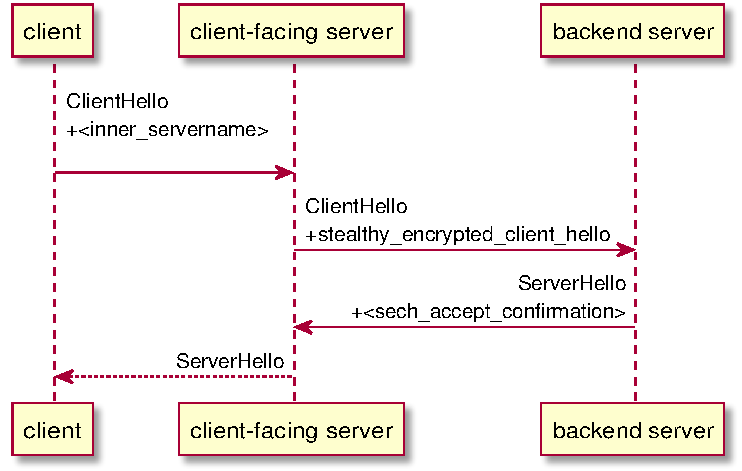
\includegraphics[width=\linewidth]{figure/sech-split-mode-accept.pdf}
\captionsetup{width=.8\linewidth} 
\caption[]{Sequence diagram for a successful SECH split-mode handshake.}
\label{fig:sech-split-mode-accept}
\end{figure}

\section{SECH 1: Secretless Stealthy Encoding}
\subsection{Motivations and Deployment Scenarios}

[ ] more properly should be called just `stealthy SNI' or `stealthy CH', because this version does not use encryption

[ ] very low coordination/infrastructure requirements to get this working

[ ] SECH.1 does **not** offer confidentiality of the SNI or ALPN, aim here is purely censorship circumvention, not privacy

[ ] as a censorship circumvention method this can be easily detected and prevented

[ ] possibly useful ephemerally and at a small scale

[ ] circumvention in depth: use lots of different circumvention methods (including this insecure one) in order to increase the cost of censorship
\subsection{Design}
\subsection{Implementation Notes}
\section{SECH 2: Static Secret Shared OOB}
\subsection{Motivations and Deployment Scenarios}

[ ] if the client and servver can share the OOB secret securely then we can implement a highly stealthy and cryptographically secure inner SNI

[ ] since the server does not have to publish a public key (as in ECH), it is possible to hide the fact that the server is support SECH from all except the client who knows the OOB secret

[ ] the secret could be shared amongst multiple clients, allowing for some scale of deployment, but this protocol is certainly not appropriate for internet scale deployments (millions of clients). The more widely the secret is shared the more likely it is to be leaked.

[ ] This design is NOT forward secret. If the shared secret is compromised then 
  - Design

[ ] assume the client and server have some way to securely share a secret out-of-band

[ ] client uses that secret to encrypt the true target server which is hidden in the ClientHello (\var{random}, \var{legacy_session_id}, \var{pre_shared_key}, grease etc.)

[ ] The client generates a 12 byte IV for AES-128-GCM. The plaintext is an ASCII encoding of the servername padded with 0x00 up to 12 bytes, which is also 8 bytes when encrypted with the 32 byte symmetric key. AEAD is used but the AAD is 0-length. The tag is truncated to 8 bytes, such that we have a combined 32 bytes to send, which is put into the ClientHello.random, the first 12 bytes contain the IV, the next 12 contain the encrypted text, and the last 8 bytes contain the truncated MAC.

[ ] If the server can decrypt and authenticate the ClientHello.random, then it proceeds to accept SECH, and makes the SECH inner servername available to the application program via a callback or some other means, which allows the application program to decide whether or not to switch contexts (server certificate etc.).

%[ ] The server uses the 32 byte shared secret key as well as the decrypted inner servername to create an 8 byte acceptance signal which is hidden in the ServerHello.random. The 8 byte acceptance signal is computed as \var{sech_accept_confirmation = AEAD-encrypt(IV, plaintext="", aad=sech_inner_servername, accept_key).tag}, where IV is the first 12 bytes of the ServerHello.random (uniformly randomly generated), the plaintext is zero-length, the AAD is precisely the inner servername (which does not need to be transmitted because it is known by the client), and \var{accept_key} is a session-specific key derived using HKDF from the session's master secret and the transcript of ClientHello..ServerHello, but with the last 16 bytes of ServerHello.random set to 0x00. The last 8 bytes of \var{ServerHello.random} are possibly used for an ECH acceptance signal, and the ECH acceptance signal is computed based on the transcript of ClientHello..ServerHello, except with the last 8 bytes of of ServerHello.random set to 0x00. Therefore, if the server is sending an SECH acceptance signal *and* an ECH acceptance signal, the SECH acceptance signal is computed first because the ECH acceptance signal is defined to incorporate the SECH acceptance signal bytes in its transcript hash. To construct the 8 sech_accept_confirmation bytes we make use of the HKDF-Expand-Label function defined in RFC 8446 Section 7.1.
    % ```c
    % md = TranscriptHash(ClientHello..ServerHello) // with last 16 bytes of ServerHello.random set to 0x00
    % padded_sech_IV = pad(sech_IV, HashLen)
    % sech_accept_confirmation = HKDF-Expand-Label(
    %   HKDF-Extract(padded_sech_IV, sech_symmetric_key),
    %   "sech ac" || 0x00 || sech_decrypted_inner_servername,
    %   md,
    %   8
    % )
    % ```

[ ] This definition of \var{sech_accept_confirmation} is essentially a modification of the ECH \var{accept_confirmation} defined in Section 7.2 of [TODO cite ECH draft], which we repeat here:
% ```
%   accept_confirmation = HKDF-Expand-Label(
%     HKDF-Extract(0, ClientHelloInner.random),
%     "ech accept confirmation",
%     transcript_ech_conf,
%     8
%   )
% ```

The ECH \var{accept_confirmation} uses \var{HKDF-Extract(0, ClientHelloInner.random)} as the `Secret' passed to \var{HKDF-Expand-Label}, and \var{HKDF-Extract(0,ClientHelloInner.random)} is confidential (only known to the client and server) because the \var{ClientHelloInner.random} was in the {\em encrypted} \var{ClientHelloInner}. Also, it is essential that \var{accept_confirmation} can be generated by the backend server in ECH split mode, which is why the salt passed to \var{HKDF-Extract} is the 0 string. While it would be more secure to use a session-specific random value as the salt for \var{HKDF-Extract}, we cannot use the \var{ClientHelloOuter.random} because this value is not available to the backend server (the backend server only processes the ClientHelloInner). The HKDF specification assumes that the salt and IKM passed to HKDF-Extract are indepedent of each other (Section 3.4 RFC 5869), and in particular that the salt values are not `chosen or manipulated by an attacker'.
Since \var{ClientHelloOuter.random} is never processed by the backend server it will not be incorporated into the \var{Finished} message, which means it is not protected from tampering in split-mode. This means an attacker could manipulate \var{ClientHelloOuter.random} and so it should not be used as the salt for \var{HKDF-Extract}.

[ ] In order to facilitate a split mode of operation in a similar fashion to ECH it must be possible for the SECH backend server to produce  the \var{sech_accept_confirmation} signal. For the signal described above this entails that the backend server must possess the \var{sech_symmetric_key}, meaning \var{sech_symmetric_key} would be shared amongst three parties; client, client-facing server, backend server. This violates one of the design requirements listed in Section 3.2 by \cite{rfc8744-issues}; Avoid Widely Shared Secrets.
% \subsection{Security Considerations}

[ ] High probability for situations where an attacker can guess the plaintext, or where there are only a small number of possible plaintexts (SNIs). How does this affect capacity to brute force the secret key? -> Does this mean the SNIs must also remain secret?

\subsection{Implementation Notes}
    - Testing
\section{SECH 3}
\subsection{Motivations and Deployment Scenarios}
\subsection{Design}
\subsection{Implementation Notes}
\section{SECH 4}
\subsection{Motivations and Deployment Scenarios}
\subsection{Design}
\subsection{Implementation Notes}
\section{SECH 5}
\subsection{Motivations and Deployment Scenarios}
\subsection{Design}
\subsection{Implementation Notes}
\section{SECH 6: TLS over TLS}
\subsection{Motivations and Deployment Scenarios}
\subsection{Design}
\subsection{Implementation Notes}


% At the beginning of each chapter, a description should introduce the reader to the content of the chapter. The description should explain to the reader the layout of the chapter, the contribution that the chapter makes to the overall dissertation and the contribution of the individual sections towards the overall chapter.


% \section{Problem Formulation}
% \label{sec:ProblemFormulation}

% This section should provide the reader with an overall description of the problem that will be addressed in the dissertation. In contrast to a generic discussion of the dissertation topic in the Introduction chapter, this section should provide a detailed discussion of the problem that has been identified based on the existing work that has been discussed in the preceeding chapter. 

% In some dissertations, it may make sense to convert this section into a short chapter of its own which follows the discussion of the existing work and preceeds the discussion of the work of the dissertation.

% \subsection{Identified Challenges}
% This section should present a short description of the gaps in the existing work and the relationship of these gaps to the work described in this dissertation.

% \subsection{Proposed Work}
% This section should provide a thorough description of the problem and an overview of the work proposed to address the problem.


% \section{Overview of the Design}
% \label{sec:OverviewOfDesign}
% A description of the approach that addresses the problem identified above.


% \section{Summary}
% \label{sec:SummaryDesign}

% Every chapter aside from the first and last chapter should conclude with a summary. 
